%% SECTION HEADER /////////////////////////////////////////////////////////////////////////////////////
\section{Excitation signal}
\label{sec:excitation}

%% SECTION CONTENT ////////////////////////////////////////////////////////////////////////////////////
A sine function modulated by the Hann window was chosen as the excitation signal.
It is defined as:
\begin{eqnarray}
	V_e(t) = 0.5\left(1-\cos(2\pi f_m(t-1/f_m)\right)\sin(2\pi f_ct),
\end{eqnarray}
\nomtypeR[freq_car]{\(f_c\)}{Carrier frequency}{}{\unit{\hertz}}%
\nomtypeR[freq_mod]{\(f_m\)}{Modulation frequency}{}{\unit{\hertz}}%
\nomtypeD[numb_cyc]{\(f_c\)}{Pulse number of cycle}{}%
where \(f_c\) is the carrier frequency, and \(f_m=f_c/N_c\) is the modulation frequency with \(N_c\) as the number of cycles.
\(N_c\) was assumed to be five, as a compromise between signal length in the time domain and signal width in the frequency domain.
It is because too high \(N_c\) may cause overlapping wave modes, while too low number will cause increasing signal dispersion.
Both issues can cause difficulties in signal processing for damage assessment.
The set of carrier frequencies was considered to be \(f_c=[50, 100, 150] \) \unit{\kHz}.
The equation of motion convergence for the model described in the following subsections was obtained with a time increment of \num{9.155e-3} \(\mu\)s.
Such a signal constitutes more than 80 \unit{\MHz} of sampling frequency.
A 5-cycle signal of 100 \unit{\kHz} is shown in Fig. \ref{fig:signal_100kHz}.
\begin{figure}[H]
	\begin{center}
		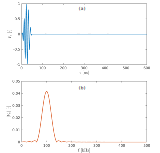
\includegraphics[width=0.95\textwidth]{Chapter_5/excitation}
	\end{center}
	\caption{The 5-cycle signal excitation at carrier frequency \(fc=100\) \unit{\kHz} \textbf{(a)} in the time domain, \textbf{(b)} in the frequency domain.}
	\label{fig:signal_100kHz}
\end{figure}
